%%%%%%%% Klassen-Optionen
\documentclass[12pt,a4paper]{scrartcl}

%%%%%%%% PAKETE: unverzichtbare Pakete mit Einstellungen
\usepackage[left=2.5cm, right=2cm, top=3cm, bottom=3cm, a4paper]{geometry} %Seitenrände
\usepackage[utf8x]{inputenc} % utf8-Kodierung und direkte Eingabe von Sonderzeichen
\usepackage{fixltx2e} % Verbessert einige Kernkompetenzen von LaTeX2e

%%%%%%%% PAKETE: AMS-Pakete
\usepackage{amsmath} % Mathe-Erweiterung
\usepackage{amsfonts} % Schrift-Erweiterung
\usepackage{amssymb} % Sonderzeichen-Erweiterung

%%%%%%%% PAKETE: Sonstiges
\usepackage[colorlinks, citecolor=black, filecolor=black, linkcolor=black, urlcolor=black]{hyperref} % Links
\usepackage{wrapfig} % ausgeklügekte Floatumgebung
\usepackage{float} % normale Floatumgebung
\restylefloat{figure} % ermöglicht die Verwendung von "H" (ist noch stärker als "h!")
\usepackage[small,it,singlelinecheck=false]{caption} % Bildunterschriften formatieren
\usepackage{multirow} % ermöglich Verbinden von Tabellenzeilen
\usepackage{multicol} % ermöglicht Spalten
\usepackage{fancyhdr} % ermöglicht Kopf- und Fußzeilen
\usepackage{graphicx} % Einbinden von Bildern möglich
\usepackage{units} % Einheiten
 \usepackage{booktabs}%Tabellen - Linien
\usepackage{subcaption}

%%%%%%%% DEFINITIONEN: Titelseite
\author{April Cooper, Patrick Kreissl und Sebastian Weber}
\title{Worksheet 3: Molecular Dynamics 2 and Observables}
\publishers{University of Stuttgart}
\date{\today}

%%%%%%%% ANPASSUNGEN: Kopf-und Fußzeile
\fancypagestyle{plain}{} % redefine the plain pagestyle to match the fancy layout
\pagestyle{fancy} % aktiviere eigenen Seitenstil
\fancyhf{} % alle Kopf- und Fußzeilen bereinigen
\fancyhead[L]{Worksheet 3:  Molecular Dynamics 2 and Observables}
\fancyhead[R]{\today}
\renewcommand{\headrulewidth}{0.6pt} % obere Trennlinie
\fancyfoot[L]{Patrick Kreissl und Sebastian Weber}
\fancyfoot[R]{Seite \thepage}
\renewcommand{\footrulewidth}{0.6pt} % untere Trennlinie

%%%%%%%% ANPASSUNGEN: Absätze
\setlength{\parindent}{0em} % keine Absatzeinzüge
\setlength{\parskip}{0em} % Absatz-Abstand

%%%%%%%% ANPASSUNGEN: Abbildungsverzeichnis
\usepackage{tocloft} % Zum Anpassen der Verzeichnisse
\renewcommand{\cftfigpresnum}{Abb. }
\renewcommand{\cfttabpresnum}{Tab. }
\renewcommand{\cftfigaftersnum}{:}
\renewcommand{\cfttabaftersnum}{:}
\setlength{\cftfignumwidth}{2cm}
\setlength{\cfttabnumwidth}{2cm}
\setlength{\cftfigindent}{0cm}
\setlength{\cfttabindent}{0cm}

%%%%%%%% SONSTIGES
\usepackage{pdfpages}
\usepackage{pgf}

% NÜTZLICH: http://truben.no/latex/table/

% Anfang des eigentlichen Dokuments
\begin{document}

\maketitle
\tableofcontents
\newpage

% =============== Section ============
\section{Functions for temperature and pressure }

We were supposed to implement \verb+compute_temperature()+ and \verb+compute_pressure()+.
\begin{itemize}
\item \verb+compute_temperature()+ was implemented in the Python-part. Because it constits of very few operations it isn't time-consuming.
\item \verb+compute_pressure()+ was implemented in the C-part. Here, you have to calculate a large sum in a large loop. Furthermore the access on the variable \verb+verlet_list+ is easier in the C-part than in the Python-part.
\end{itemize}



\section{Running averages}
In this section we had to calculate the running averages of the measured observables.
The resulting plot can be  seen below:
\begin{figure}[H]
\centering
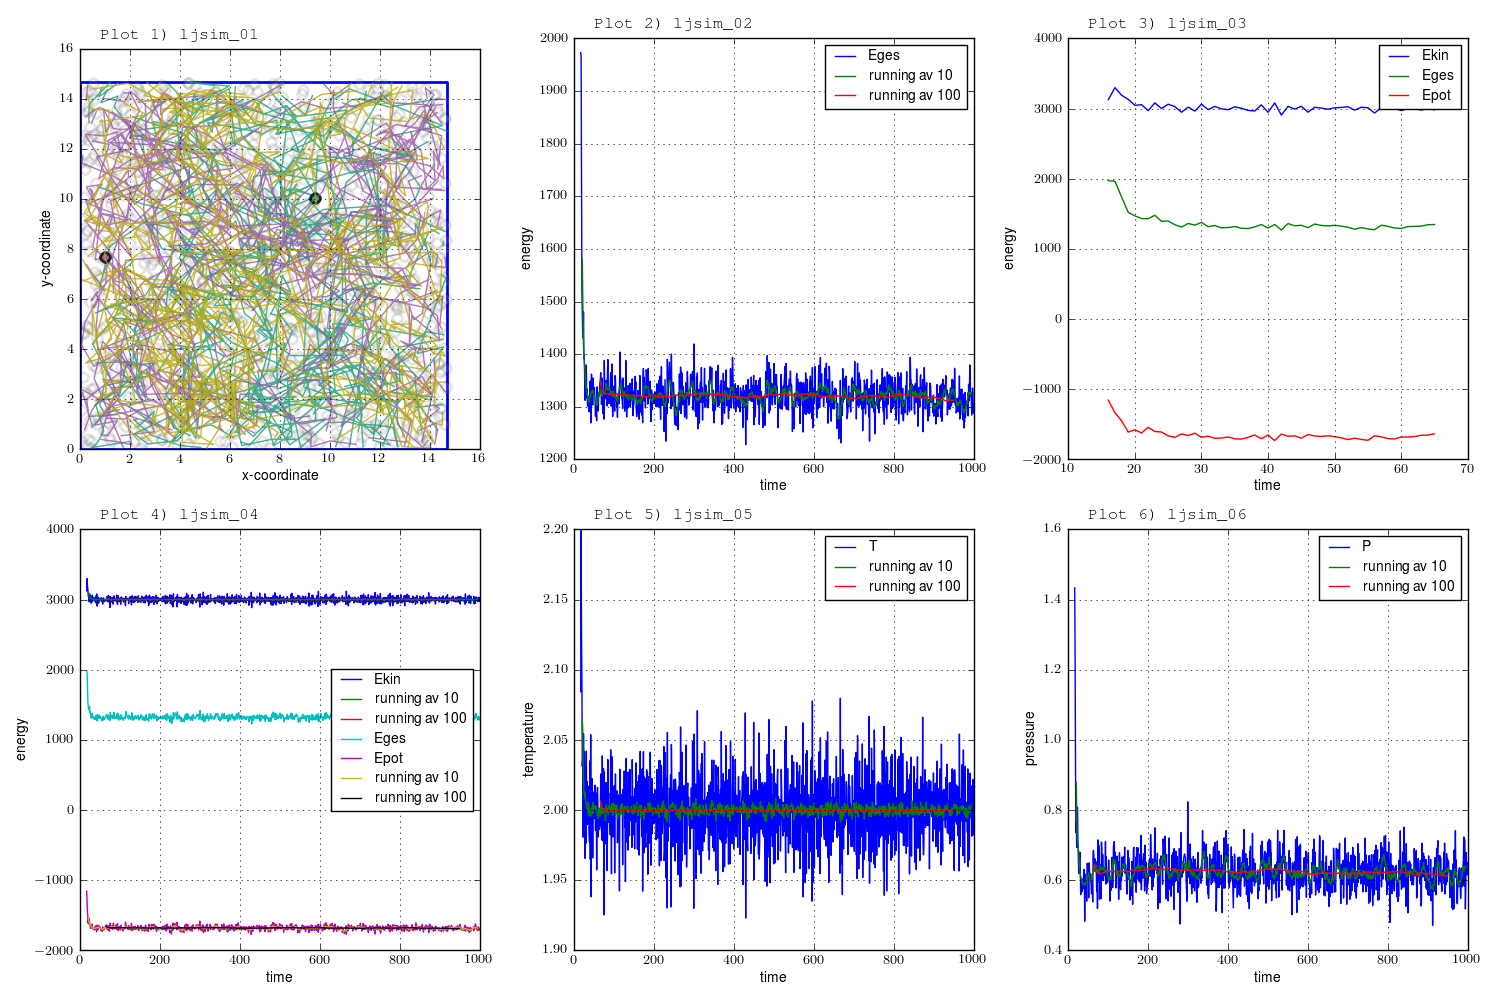
\includegraphics[width=16.0cm]{../plots/t1000.png}
\caption{Observables up to t=1000 and their running averages}
\label{fig:running averages}
\end{figure}

It can be observed that the observables fluctuate during the first time steps immensely and after some time they still fluctuate a bit, but their mean values become quite constant. This is due to the fact that first the system is equilibrating wherefore the observables fluctuate quite much, after this process the system is in equilibrium and therefore the observables stay constant.
The time the system needs to be equilibrated is about $t_equi=20$ time units.
This can be easily seen as all the following graphs and especially all running averages showing a rather constant behavior .
\begin{figure}[H]
\centering
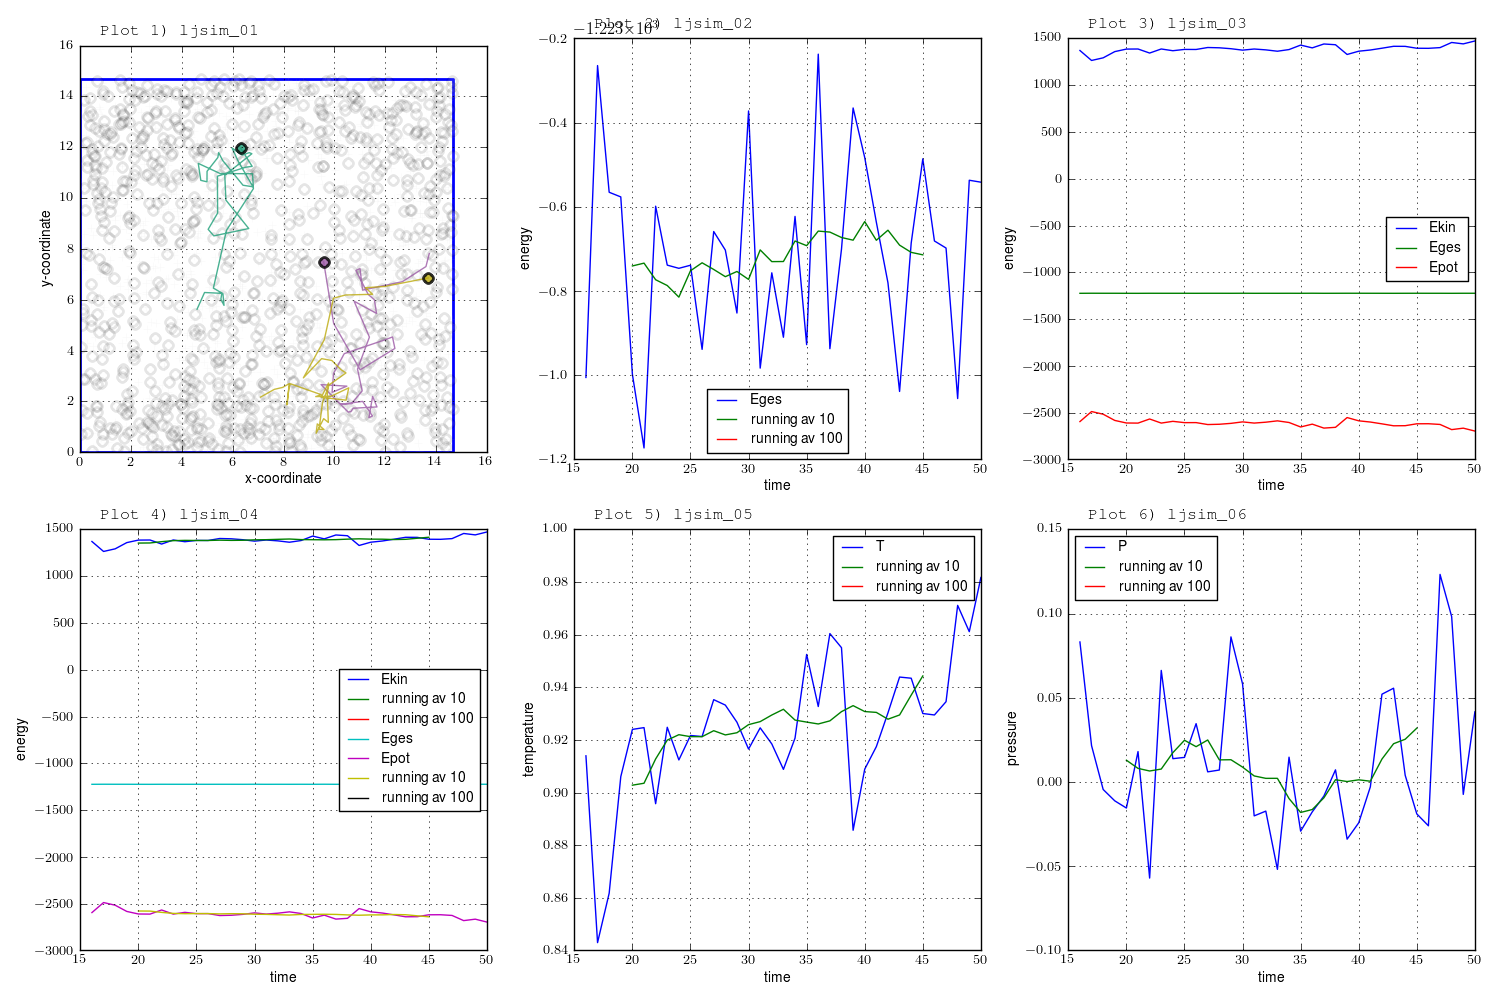
\includegraphics[width=16.0cm]{../plots/Tequi.png}
\caption{Observables up to t=1000 and their running averages}
\label{fig:running averages}
\end{figure}

In this context it should be mentioned, that there is no running average for window size 100 as we only simulated 50 time steps.
The mean values of the observables measured in one of our simulatios are:\newline
\begin{center}
\begin{tabular}{cc}
\toprule
Observable & Mean value\\
\midrule
$E_{tot}$&1329.25\\
$E_{pot}$&-1671.12\\
$E_{kin}$&3000.38\\
T&2.00\\
P&0.6\\
\bottomrule
\end{tabular}
\end{center}

\section{Velocity rescaling}
 \subsection{Derivation of the rescaling factor}
 It is: 
 \begin{equation}
 \frac{k_bT}{2}=\frac{0.5mv^2}{3N}
 \end{equation}
 Which obviously leads to:
  \begin{equation}\nonumber
 T_{mes}=\frac{mv_{mes}^2}{3Nk_B} \\
 \end{equation}
\begin{equation}\nonumber
  T_{des}=\frac{mv_{des}^2}{3Nk_B} \\
\end{equation}
where $T_{mes}$ is the measured and $T_{des}$ is the desired temperature - analogous for the velocities.
Calculating the factor $\frac{T_{mes}}{T_{des}}$ and solving for $v_{des}$ leads to:
\begin{equation}
v_{des}=v_{mes} \sqrt{\frac{T_{des}}{T_{mes}}}
\end{equation}
Therefore you have to multiply the measured velocities $v_{mes}$ by the factor $\sqrt{\frac{T_{des}}{T_{mes}}}$ in order to get a correct velocity rescaling.
\newline
\newline
This velocity rescaling has been implemented in the python part due to the fact that it's a simple multiplication with a factor and nothing numerically problematic. Implementing it in C had only made this calculation more komlpex to implement and wouldn't bring a big simulation time reduction.
The plots of all observables for $T_{des}$ = 0.3, 1.0 and 2.0 are the following:
\begin{figure}[H]
\centering
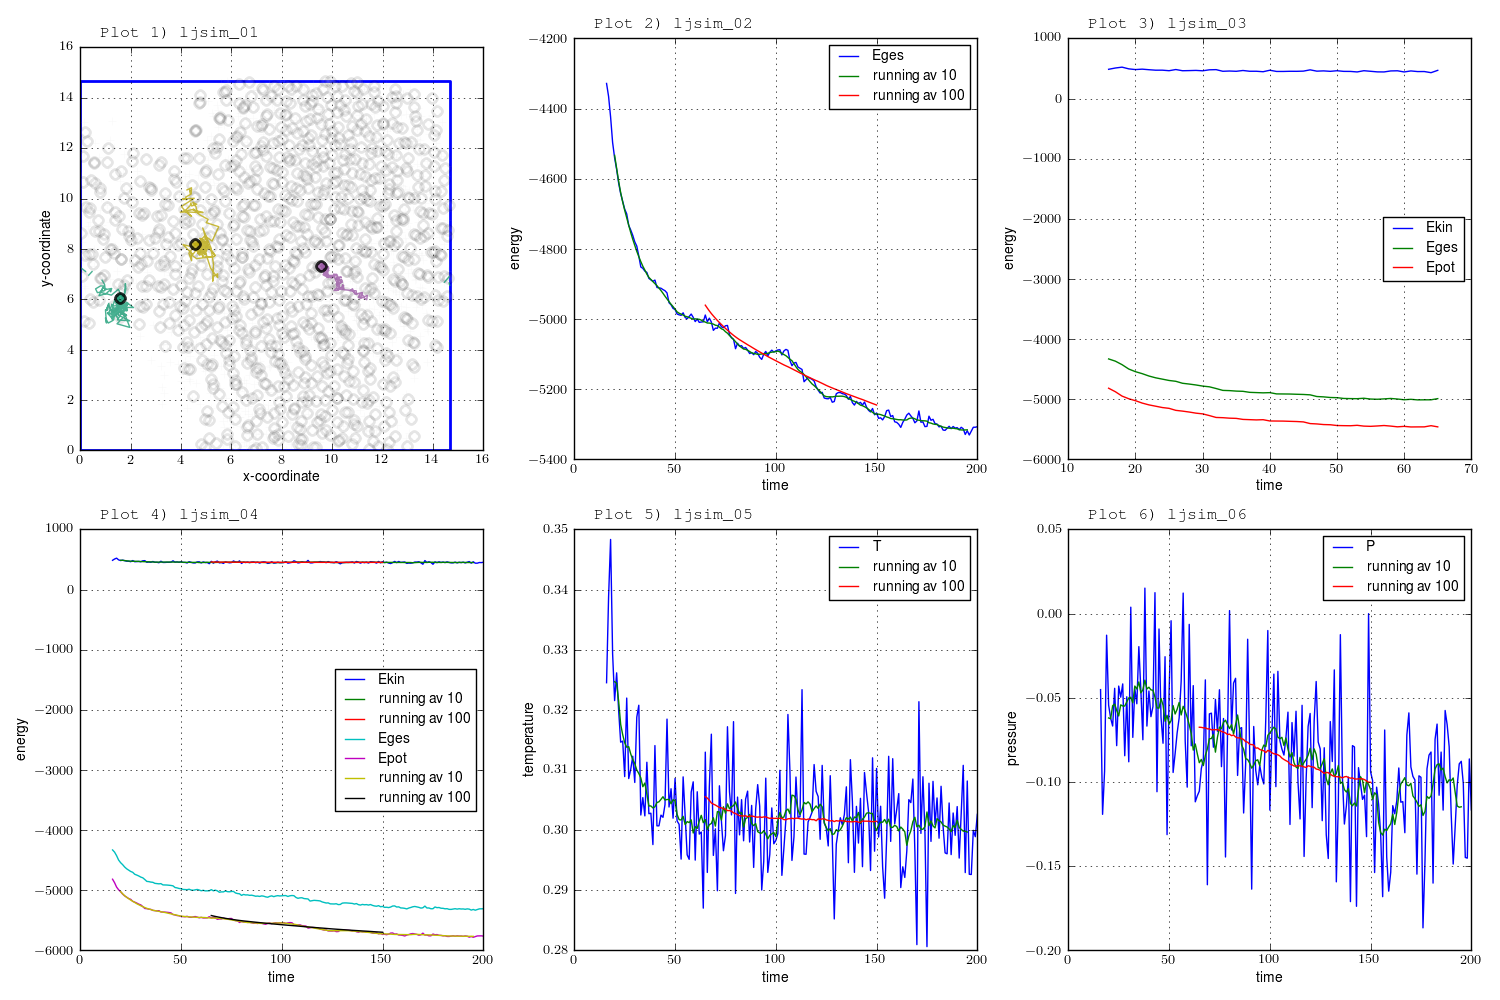
\includegraphics[width=16.0cm]{../plots/Tdes03.png}
\caption{Observables for $T_{des}$ = 0.3 and their running averages}
\label{fig:running averages Tdes03}
\end{figure}
\begin{figure}
\centering
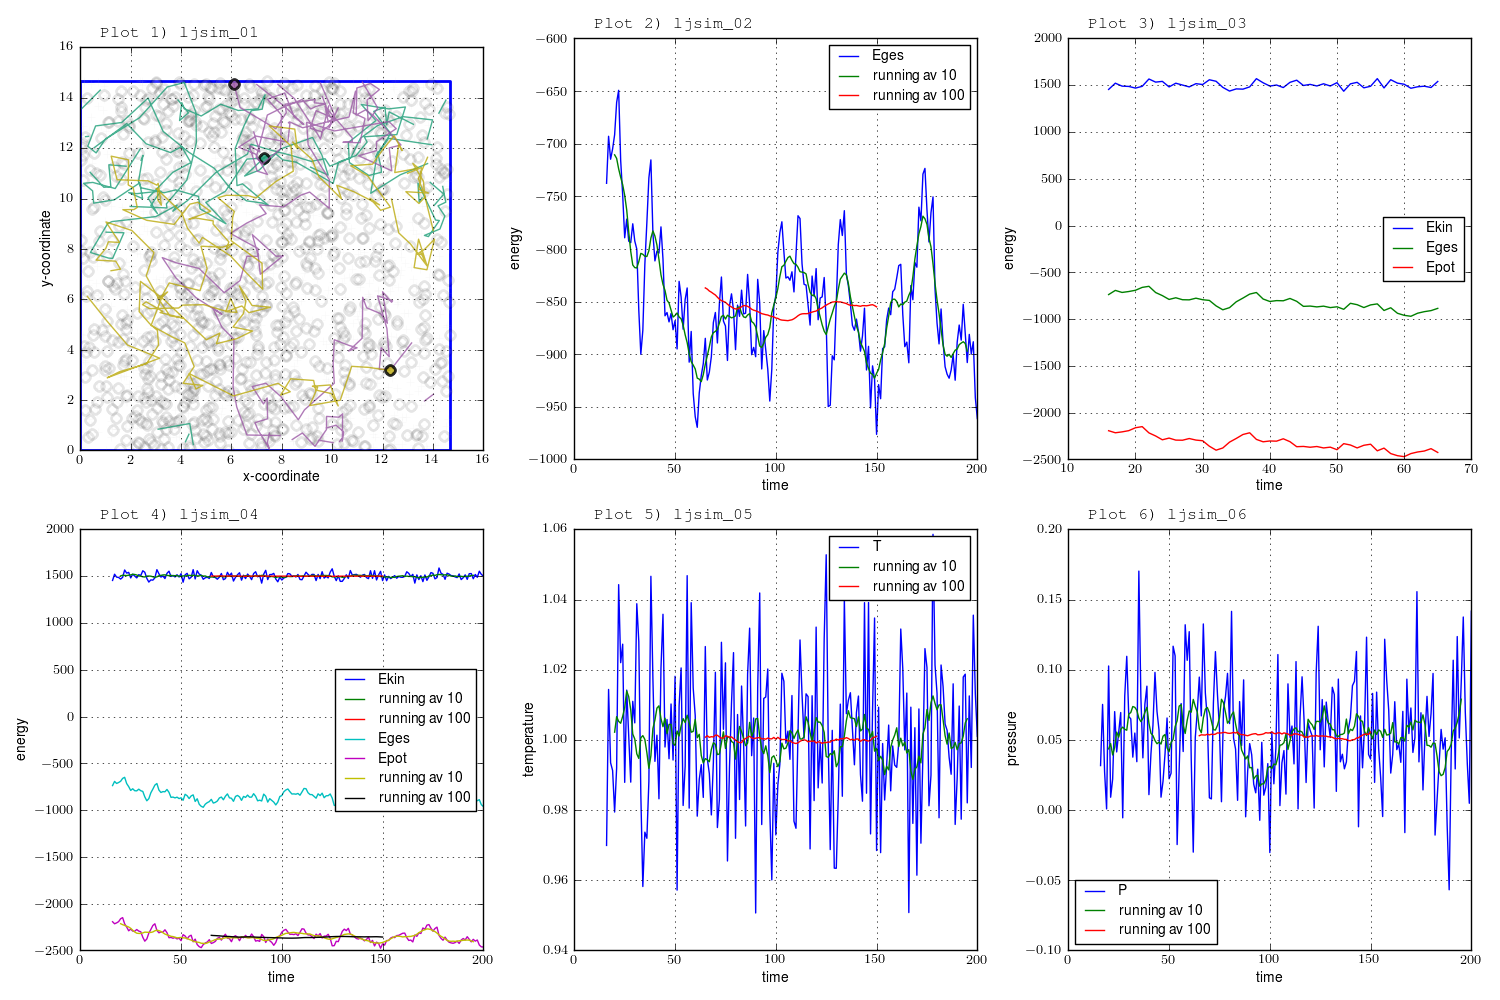
\includegraphics[width=16.0cm]{../plots/Tdes1.png}
\caption{Observables for $T_{des}$ = 1.0 and their running averages}
\label{fig:running averages Tdes1} 
\end{figure}
\begin{figure}[H]
\centering
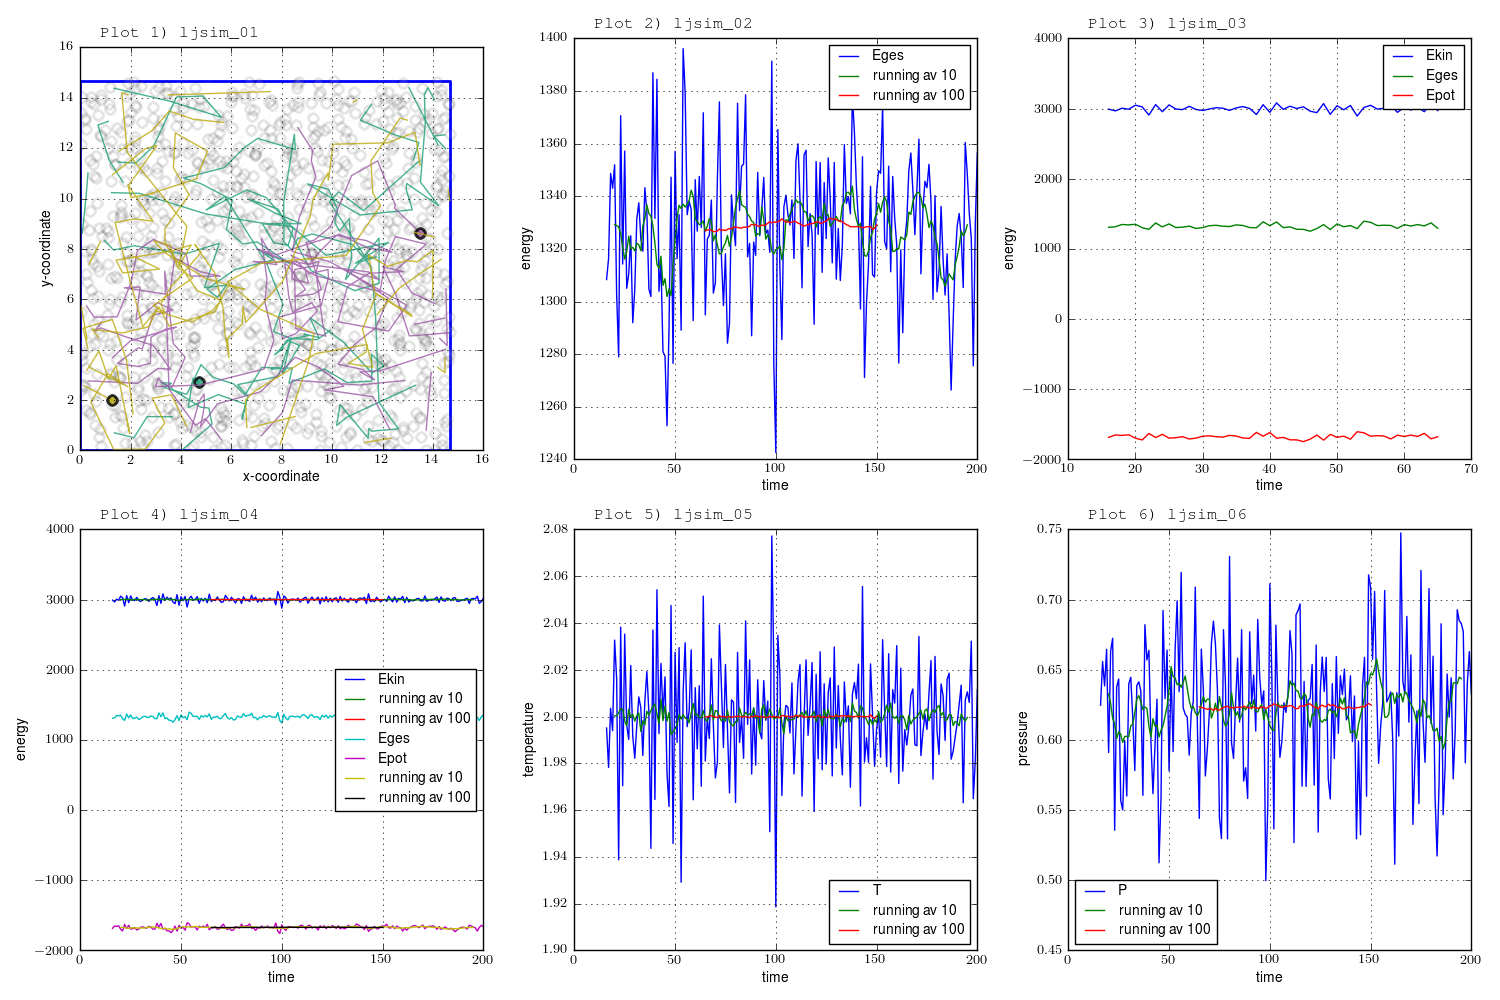
\includegraphics[width=16.0cm]{../plots/Tdes2.png}
\caption{Observables for $T_{des}$ = 2.0 and their running averages}
\label{fig:running averages Tdes2}
\end{figure}
Comparing these three plots it can easily be seen that the total energies increase with the temperature which would be expected, due to the fact that the kinetic energy will increase with temperature.
It also seems that equilibration will take longer for lower temperatures which can be explained by the lower average kinetic energy and therefore averagely slower movement of the particles.

\section{Force capping}
Force capping was implemented in C-part because it belongs in the function \verb+c_compute_forces+. In addition it's a more or less complex operation when you want to do it the right way (the simple way would by to do force capping component by component).

It's important to rescale the velocities regularly when you use force capping. In addition the initially calculated observables contain large errors so that you have to reject them for analyzing. If you give attention to both of these aspects, the new set up will work well.

\section{Plots with RDF}
\subsection*{For T=0.3}
\includegraphics[page=1, scale=0.6]{../plots/plots_T03}
\subsection*{For T=1.0}
\includegraphics[page=1, scale=0.6]{../plots/plots_T10}
\subsection*{For T=2.0}
\includegraphics[page=1, scale=0.6]{../plots/plots_T20}

\end{document}

% =============== Comments ============
\verb+x_init {}+

\begin{figure}[H]
	\resizebox{1\textwidth}{!{\input{../plots/NAME.pgf}}
	\caption{CAPTION}\label{fig:NAME}
\end{figure}
